
\section{MIC implementation}
One of the most important factors to take into consideration when implementing PV modules is to obtain the maximum energy possible out of the available hardware, if this is not done, energy that should have been obtained will instead be lost. Since energy is equal to power over time, power must be maximized when the energy is being extracted. To achieve such goal a maximum power point tracker needs to be implemented. This is an electrical system that is always on the search of the location of the point where power extraction can be peaked. 

MPPTs mostly consist of a power circuit that regulates either voltage drop or current flow across the PV terminals. There are many kinds of circuits that can be used to follow the MPP of the PV, this topic will be further introduced in chapter \ref{background}.
However, solar plants and domestic installations are composed of many modules, these modules are then connected to each other in series or parallel configurations. To simplify the system, one MPPT is commonly used for many modules, this approach may lead to imperfections in the efficiency rates since the uneven power generation might lead to have a system with local MPP in addition to the global MPP. In figure \ref{multiple_local_MPP} a system exhibiting 2 MPP is shown. In order to ensure that the system is working in the global MPP and not in a local MPP, the controller will have to perform a voltage sweep. This voltage sweep is a higher level of complexity in the MPPT control system. In any case, the system will not be able to get the actual power generation, as one panel is bypassed by a diode.

\begin{figure}[htbp]
	\begin{center}
		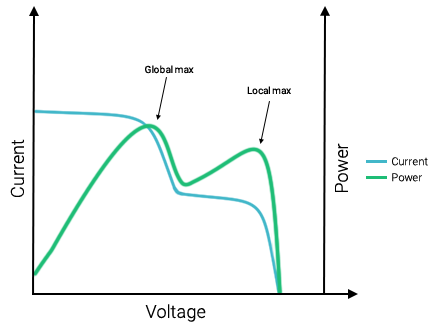
\includegraphics[width=0.6\textwidth]{../Pictures/local_MPP}
		\caption{I-V curve of a system with more than one MPP. The cause is partial shading \cite{local_mpp}.}
		\label{multiple_local_MPP}
	\end{center}	
\end{figure}

Using MICs for each module results in higher overall efficiencies, with this technology, events like partial shading, uneven dirt, wear distribution or imperfections produced in the assembly line are reduced and do not effect the rest of the modules in a line. Also, a more detailed control of the plant is achieved since separate data from each individual panel is obtained.
Different implementation options for MIC devices are possible but the most important objective of these devices is to individually control each module, resulting on an overall better efficiency rate, as well as a more robust system against any kind of disturbance. Each PV module will then be connected directly to each MIC, with this setup the output voltage and current are regulated by the device that extracts the energy, either an inverter, a battery or a load, allowing the system to work at different voltage and current levels whilst maintaining the MPP at all time. 

MICs can be divided in microinverters and DC-DC. In figure \ref{MIC_dcdc} a system using MICs to perform the voltage reduction or increase is used. Notice that $N$ panels might be used. All MICs' output is connected to the general inverter input. The power rating of this DC-AC will have to be higher than the maximum power that can be delivered by MICs. Then the size of the inverter must consider the amount of PV panels installed.

\begin{figure}[htbp]
	\begin{center}
		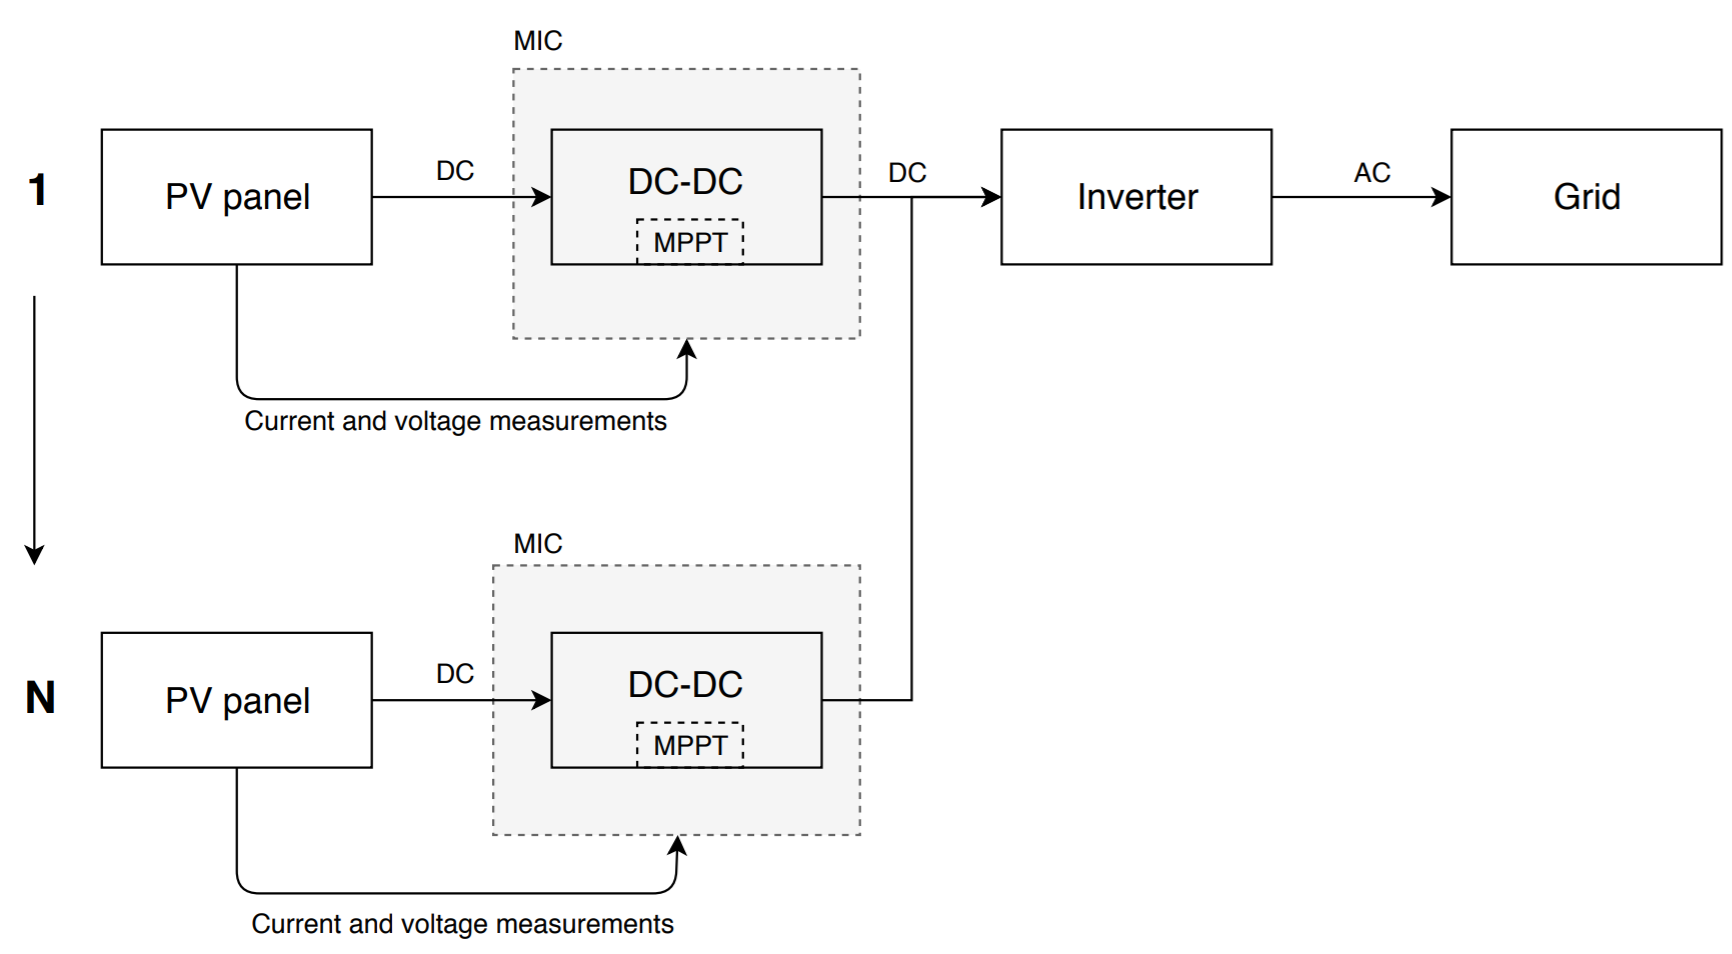
\includegraphics[width=0.7\textwidth]{../Pictures/MIC_dcdc}
		\caption{PV generation with DC-DC MIC system structure.}
		\label{MIC_dcdc}
	\end{center}	
\end{figure}

The panels with a MIC consisting on a microinverter, include a DC-DC and are directly tied to grid. In figure \ref{microinverter_system} a microinverter system structure can be seen. For the user, this system is simpler, as only the PV must be purchased. The user doesn't have to worry about selecting and installing an inverter. 

\begin{figure}[htbp]
	\begin{center}
		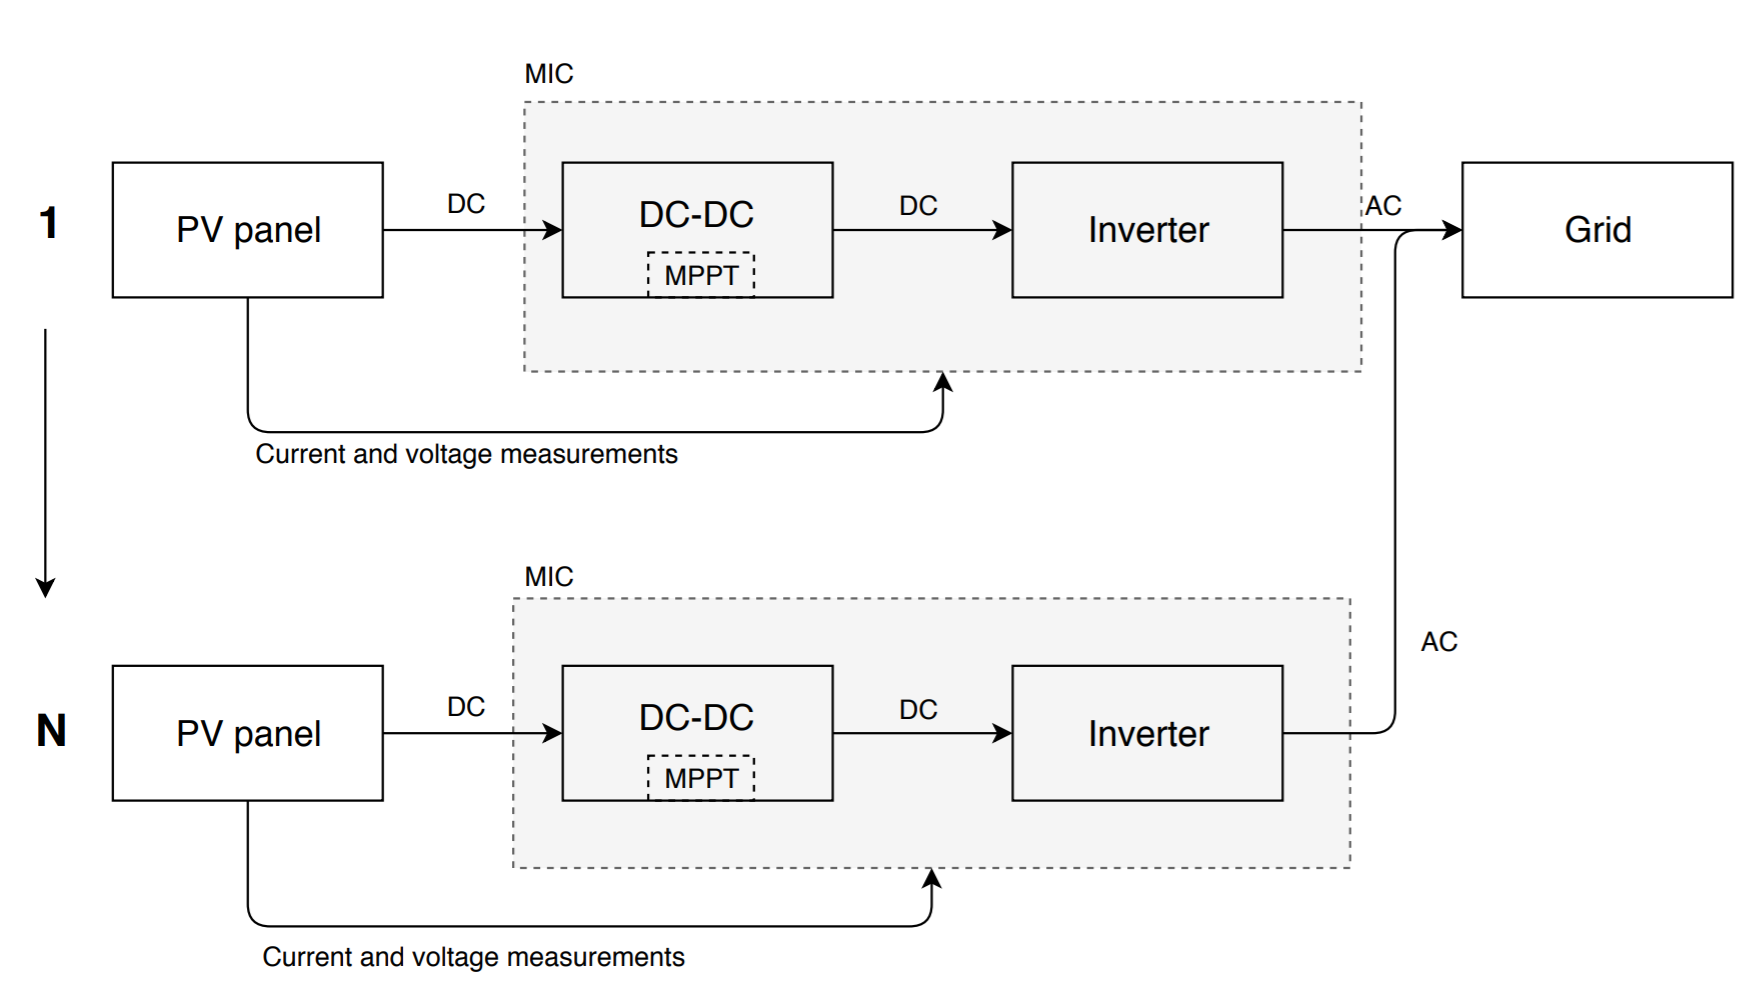
\includegraphics[width=0.7\textwidth]{../Pictures/MIC_microinverter}
		\caption{PV generation with microinverter MIC system structure.}
		\label{microinverter_system}
	\end{center}	
\end{figure}
The main advantages of the microinverter system is that it is simpler for the user however it implies cost increase and are usually less efficient than a DC-DC system with a higher power general inverter \cite{ArchitectureMIC}, then a DC-DC MIC will be developed. 


